\chapter{Descretization of the dynamics}
{\bf \Large 
\begin{tabular}{ccc}
\hline
  Corresponding author & : & Hirofumi Tomita\\
\hline
\end{tabular}
}

\section{Time integration method}

For the time integration of Eqs.(\ref{eq:rhotot_d2})-(\ref{eq:etot_d2}),
we adopt the full explicit scheme with
the $p$-th order Runge-Kutta scheme.
\begin{eqnarray}
&&  \phi^{*} = \phi^{t} - \left(\frac{\partial \phi}{\partial t}\right)^{t}\frac{\Delta t}{p}\\
&&  \phi^{**} = \phi^{t} - \left(\frac{\partial \phi}{\partial t}\right)^{*}\frac{\Delta t}{p-1}\\
&&  \cdot \cdot \cdot\nonumber\\
&&  \cdot \cdot \cdot\nonumber\\
&&  \cdot \cdot \cdot\nonumber\\
&&  \phi^{t+\Delta t} = \phi^{t} - \left(\frac{\partial \phi}{\partial t}\right)^{**\cdot\cdot\cdot\cdot*} \Delta t
\end{eqnarray}
Usually, we use $p=2,3$ and $4$.

%% HEVE full explicit
%% HEVI 
%% HIVI full implicit

\section{Spatial descretization}
We employ the Arakawa-C staggered grid with the 3-dimensional momentum 
($\rho u, \rho v, \rho w$), density ($\rho$) and mass-weighted potentail temperature($\rho \theta$)
as the prognostic variables.
Figure \ref{fig:cntrl-volume}(a) shows the structure of the control volume for the mass,
indicating the location of each of prognostic variables.
Conceptually, we use the 4th order central difference scheme 
for the advection or convection terms and
the 2nd order central difference scheme for the other terms.
Before the descretization of differential equations,
we should diagnose several quantities from the prognostic variables.
\begin{description}
\item[Full-level pressure and potential temperature]
\begin{eqnarray}
&&p_{i,j,k}=p_{00}\left[\frac{(\rho \theta)_{i,j,k} R^*}{p_{00}} \right]^{\frac{c_{p}^*}{c_{p}^*- R^*}}\\
&&\theta_{i,j,k} = \frac{(\rho \theta)_{i,j,k}}{\rho_{i,j,k}}\\
\end{eqnarray}
\item[Half-level density]
\begin{eqnarray}
&&  \overline{\rho}_{i+\frac{1}{2},j,k} = \frac{\rho_{i+1,j,k}+\rho_{i,j,k}}{2}\\
&&  \overline{\rho}_{i,j+\frac{1}{2},k} = \frac{\rho_{i,j+1,k}+\rho_{i,j,k}}{2}\\
&&  \overline{\rho}_{i,j,k+\frac{1}{2}} = \frac{\rho_{i,j,k+1}+\rho_{i,j,k}}{2}\\
\end{eqnarray}
\item[Half-level velocity]
\begin{eqnarray}
&&  \overline{u}_{i+\frac{1}{2},j,k} = \frac{(\rho u)_{i+\frac{1}{2},j,k}}{\overline{\rho}_{i+\frac{1}{2},j,k}}\\
&&  \overline{v}_{i,j+\frac{1}{2},k} = \frac{(\rho v)_{i,j+\frac{1}{2},k}}{\overline{\rho}_{i,j+\frac{1}{2},k}}\\
&&  \overline{w}_{i,j,k+\frac{1}{2}} = \frac{(\rho w)_{i,j,k+\frac{1}{2}}}{\overline{\rho}_{i,j,k+\frac{1}{2}}}
\end{eqnarray}
\item[Full-level velocity]
\begin{eqnarray}
&&  \overline{u}_{i,j,k} = \frac{(\rho u)_{i+\frac{1}{2},j,k}+(\rho u)_{i-\frac{1}{2},j,k}}{2\rho_{i,j,k}}\\
&&  \overline{v}_{i,j,k} = \frac{(\rho v)_{i,j+\frac{1}{2},k}+(\rho v)_{i,j-\frac{1}{2},k}}{2\rho_{i,j,k}}\\
&&  \overline{w}_{i,j,k} = \frac{(\rho w)_{i,j,k+\frac{1}{2}}+(\rho w)_{i,j,k-\frac{1}{2}}}{2\rho_{i,j,k}}
\end{eqnarray}
\end{description}




\subsection{Continuity equation}
\begin{eqnarray}
%%
\left(\frac{\partial \rho}{\partial t}\right)_{i,j,k}
&=& - \frac{(\rho u)_{i+\frac{1}{2},j,k} -(\rho u)_{i-\frac{1}{2},j,k}}{\Delta x}\nonumber\\
& & - \frac{(\rho v)_{i,j+\frac{1}{2},k} -(\rho v)_{i,j-\frac{1}{2},k}}{\Delta y}\nonumber\\
& & - \frac{(\rho w)_{i,j,k+\frac{1}{2}} -(\rho w)_{i,j,k-\frac{1}{2}}}{\Delta z}
\end{eqnarray}

\subsection{Momentum equations}
Figure \ref{fig:cntrl-volume}(a) shows the structure of the control volume for the momentum
in the x direction.
The momentum equation is descretized as
\begin{eqnarray}
%%
\left(\frac{\partial \rho u}{\partial t}\right)_{i+\frac{1}{2},j,k}
&=& - \frac{\overline{(\rho u)}_{i+1,j,k} \overline{u}_{i+1,j,k} 
           -\overline{(\rho u)}_{i,j,k} \overline{u}_{i,j,k}}
     {\Delta x}\nonumber\\
& & - \frac{\overline{(\rho u)}_{i+\frac{1}{2},j+\frac{1}{2},k}  \overline{v}_{i+\frac{1}{2},j+\frac{1}{2},k} 
           -\overline{(\rho u)}_{i+\frac{1}{2},j-\frac{1}{2},k}  \overline{v}_{i+\frac{1}{2},j-\frac{1}{2},k}}
     {\Delta y}\nonumber\\
& & - \frac{\overline{(\rho u)}_{i+\frac{1}{2},j,k+\frac{1}{2}}  \overline{v}_{i+\frac{1}{2},j,k+\frac{1}{2}} 
           -\overline{(\rho u)}_{i+\frac{1}{2},j,k-\frac{1}{2}}  \overline{v}_{i+\frac{1}{2},j,k-\frac{1}{2}}}
     {\Delta z}\nonumber\\
& & -\frac{p_{i+1,j,k}-p_{i,j,k}}{\Delta x},
\end{eqnarray}
where 
\begin{eqnarray}
&& \overline{(\rho u)}_{i,j,k} \nonumber\\
= && \frac{-(\rho u)_{i+\frac{3}{2},j,k}+7(\rho u)_{i+\frac{1}{2},j,k}+7(\rho u)_{i-\frac{1}{2},j,k}-(\rho u)_{i-\frac{3}{2},j,k}}{12}\\
&& \overline{(\rho u)}_{i+\frac{1}{2},j+\frac{1}{2},k} \nonumber\\
= && \frac{-(\rho u)_{i+\frac{1}{2},j+2,k}+7(\rho u)_{i+\frac{1}{2},j+1,k}+7(\rho u)_{i+\frac{1}{2},j,k}-(\rho u)_{i+\frac{1}{2},j-1,k}}{12}\\
&& \overline{(\rho u)}_{i+\frac{1}{2},j,k+\frac{1}{2}} \nonumber\\
= &&\frac{-(\rho u)_{i+\frac{1}{2},j,k+2}+7(\rho u)_{i+\frac{1}{2},j,k+1}+7(\rho u)_{i+\frac{1}{2},j,k}-(\rho u)_{i+\frac{1}{2},j,k-1}}{12}
\end{eqnarray}
and the velocities at the cell wall for the staggered control volume to $x$ direction are
defined as
\begin{eqnarray}
\overline{u}_{i,j,k} &=& \frac{\overline{u}_{i+\frac{1}{2},j,k}+\overline{u}_{i-\frac{1}{2},j,k}}{2}\\
\overline{v}_{i+\frac{1}{2},j+\frac{1}{2},k} &=& 
\frac{\overline{v}_{i,j+\frac{1}{2},k}+\overline{v}_{i+1,j+\frac{1}{2},k}}{2}\\
\overline{w}_{i+\frac{1}{2},j,k+\frac{1}{2}} &=& 
\frac{\overline{w}_{i,j,k+\frac{1}{2}}+\overline{w}_{i+1,j,k+\frac{1}{2}}}{2}
\end{eqnarray}
In this form, the 4th order accuracy is guaranteed 
on the condition of the constant velocity.

The momentum equations in the $y$ and $z$ directions are descretized 
in the same way:
\begin{eqnarray}
%%
\left(\frac{\partial \rho v}{\partial t}\right)_{i,j+\frac{1}{2},k}
&=& - \frac{\overline{(\rho v)}_{i+\frac{1}{2},j+\frac{1}{2},k}  \overline{u}_{i+\frac{1}{2},j+\frac{1}{2},k} 
           -\overline{(\rho v)}_{i-\frac{1}{2},j+\frac{1}{2},k}  \overline{u}_{i-\frac{1}{2},j+\frac{1}{2},k}}
     {\Delta x}\nonumber\\
& & - \frac{\overline{(\rho v)}_{i,j+1,k} \overline{v}_{i,j+1,k} 
           -\overline{(\rho v)}_{i,j,k} \overline{v}_{i,j,k}}
     {\Delta y}\nonumber\\
& & - \frac{\overline{(\rho v)}_{i,j+\frac{1}{2},k+\frac{1}{2}}  \overline{v}_{i,j+\frac{1}{2},k+\frac{1}{2}} 
           -\overline{(\rho v)}_{i,j+\frac{1}{2},k-\frac{1}{2}}  \overline{v}_{i,j+\frac{1}{2},k-\frac{1}{2}}}
     {\Delta z}\nonumber\\
& & -\frac{p_{i,j+1,k}-p_{i,j,k}}{\Delta y},\\
%%
\left(\frac{\partial \rho w}{\partial t}\right)_{i,j,k+\frac{1}{2}}
&=& - \frac{\overline{(\rho w)}_{i+\frac{1}{2},j,k+\frac{1}{2}}  \overline{u}_{i+\frac{1}{2},j,k+\frac{1}{2}} 
           -\overline{(\rho w)}_{i-\frac{1}{2},j,k+\frac{1}{2}}  \overline{u}_{i-\frac{1}{2},j,k+\frac{1}{2}}}
     {\Delta x}\nonumber\\
& & - \frac{\overline{(\rho w)}_{i,j+\frac{1}{2},k+\frac{1}{2}}  \overline{w}_{i,j+\frac{1}{2},k+\frac{1}{2}} 
           -\overline{(\rho w)}_{i,j-\frac{1}{2},k+\frac{1}{2}}  \overline{w}_{i,j-\frac{1}{2},k+\frac{1}{2}}}
     {\Delta y}\nonumber\\
& & - \frac{\overline{(\rho w)}_{i,j,k+1} \overline{w}_{i,j,k+1} 
           -\overline{(\rho w)}_{i,j,k} \overline{w}_{i,j,k}}
     {\Delta z}\nonumber\\
& & -\frac{p_{i,j,k+1}-p_{i,j,k}}{\Delta z}-\overline{\rho}_{i,j,k+\frac{1}{2}} g
\end{eqnarray}

\subsection{Energy equation}

\begin{eqnarray}
%%
\left(\frac{\partial \rho \theta}{\partial t}\right)_{i,j,k}
&=& - \frac{(\rho u)_{i+\frac{1}{2},j,k} \overline{\theta}_{i+\frac{1}{2},j,k} 
           -(\rho u)_{i-\frac{1}{2},j,k} \overline{\theta}_{i-\frac{1}{2},j,k}}
     {\Delta x}\nonumber\\
& &  - \frac{(\rho v)_{i,j+\frac{1}{2},k} \overline{\theta}_{i,j+\frac{1}{2},k} 
           -(\rho v)_{i,j-\frac{1}{2},k} \overline{\theta}_{i,j-\frac{1}{2},k}}
     {\Delta y}\nonumber\\
& &  - \frac{(\rho w)_{i,j,k+\frac{1}{2}} \overline{\theta}_{i,j,k+\frac{1}{2}} 
           -(\rho w)_{i,j,k-\frac{1}{2}} \overline{\theta}_{i,j,k-\frac{1}{2}}}
     {\Delta z}\nonumber\\
\end{eqnarray}
where
\begin{eqnarray}
&& \overline{\theta}_{i+\frac{1}{2},j,k} = 
\frac{-\theta_{i+2,j,k}+7\theta_{i+1,j,k}+7\theta_{i,j,k}-\theta_{i-1,j,k}}{12}\\
&& \overline{\theta}_{i,j+\frac{1}{2},k} = 
\frac{-\theta_{i,j+2,k}+7\theta_{i,j+1,k}+7\theta_{i,j,k}-\theta_{i,j-1,k}}{12}\\
&& \overline{\theta}_{i,j,k+\frac{1}{2}} = 
\frac{-\theta_{i,j,k+2}+7\theta_{i,j,k+1}+7\theta_{i,j,k}-\theta_{i,j,k-1}}{12}
\end{eqnarray}

\subsection{Tracer advection}
{\Huge TBD}
description of CWC and FCT. 

\section{boundary condition}
The boundary condition only for the vertical velocity at the top and bottom
boundaries is needed:
\begin{eqnarray}
&&  w_{i,j,k_{max}+\frac{1}{2}} = 0\\
&&  w_{i,j,k_{min}-\frac{1}{2}} = 0
\end{eqnarray}
This leads to the boundary condition of the prognostic variable as
\begin{eqnarray}
&&  (\rho w)_{i,j,k_{max}+\frac{1}{2}} = 0\\
&&  (\rho w)_{i,j,k_{min}-\frac{1}{2}} = 0
\end{eqnarray}



\section{Numerical filters}

We impose no explicit numerical filter.
The numerical stability can be achieved
by aid of tiny portion of turbulence scheme.


\begin{figure}[t]
\begin{center}
  \begin{tabular}{l}
    (a) Control volume for the mass\\
  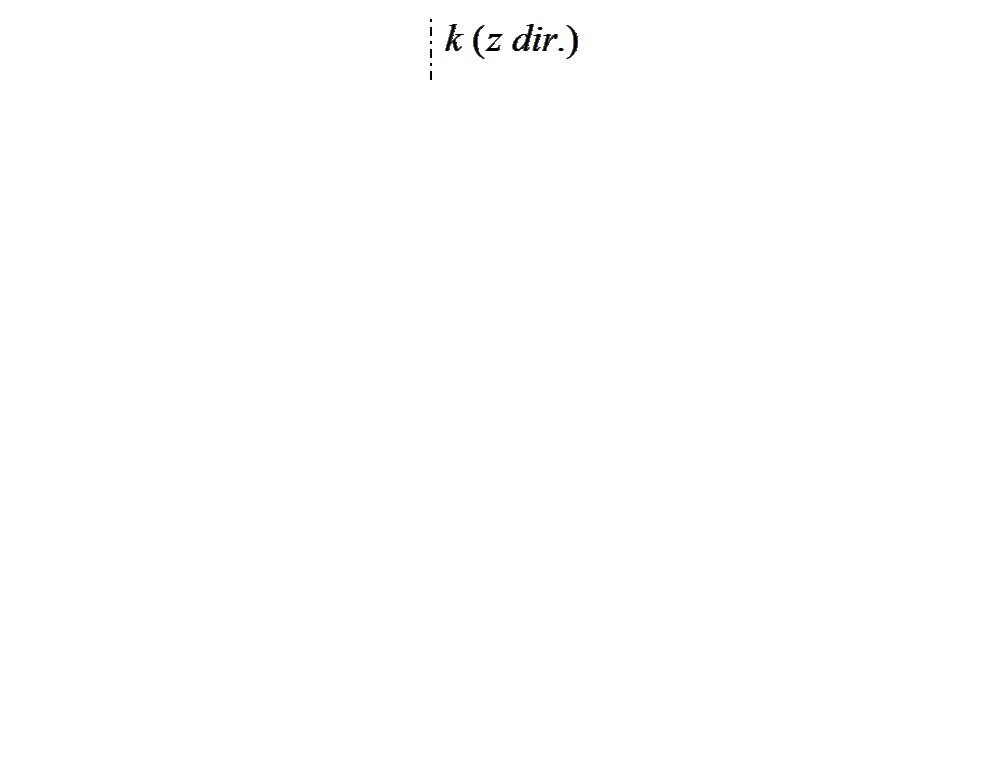
\includegraphics[scale=0.6]{./figure/cntrl-volume.eps}\\
    (b) Control volume for the momentum\\
  \includegraphics[scale=0.6]{./figure/cntrl-volume2.eps}\\
  \end{tabular}
\end{center}
  \caption{Control volume}
  \label{fig:cntrl-volume}
\end{figure}
